%%%%%%%%%%%%%%%%%%%%%%%%%%%%%%%%%%%%%%%%%%%%%%
%                insertmeeting
% 1) Title (something creative & funny?)
% 2) Date (MM/DD/YYYY)
% 3) Location (ex. Hagerty High School)
% 4) People/Committees Present 
% 5) Picture 
% 6) Start Time & Stop Time (ex. 12:30AM to 4:30PM)
%%%%%%%%%%%%%%%%%%%%%%%%%%%%%%%%%%%%%%%%%%%%%%
\insertmeeting 
	{Organizing Outreach} 
	{08/18/21}
	{Hagerty High School}
	{Annika, Falon, Jensen, Nathan, Ritam, Rose, Samantha}
	{Images/RobotPics/robot.jpg}
	{1:30 - 4:30}
	
\subsection*{Outreach}
\noindent\hfil\rule{\textwidth}{.4pt}\hfil
\subsubsection*{Goals}
\begin{itemize}
    \item Discuss future plans for Outreach and come up with more challenging/unique outreach opportunities for our team.  

\end{itemize} 

\noindent\hfil\rule{\textwidth}{.4pt}\hfil

\subsubsection*{Accomplishments}
We started off by throwing random ideas back and forth, while refreshing our memories on which events have worked well for us in the past. Someone suggested that we could do teaching sessions with the 4227 members for specific skills like multimedia or CAD. This seems like a pretty good idea, and we will probably try to do this throughout the rest of the pre-season period. Then, we want to try and do more events at public spaces like Publix and possibly try to make it a hands-on experience for younger people.

\begin{figure}[htp]
\centering
\begin{minipage}[b]{.50\textwidth}
  \centering
  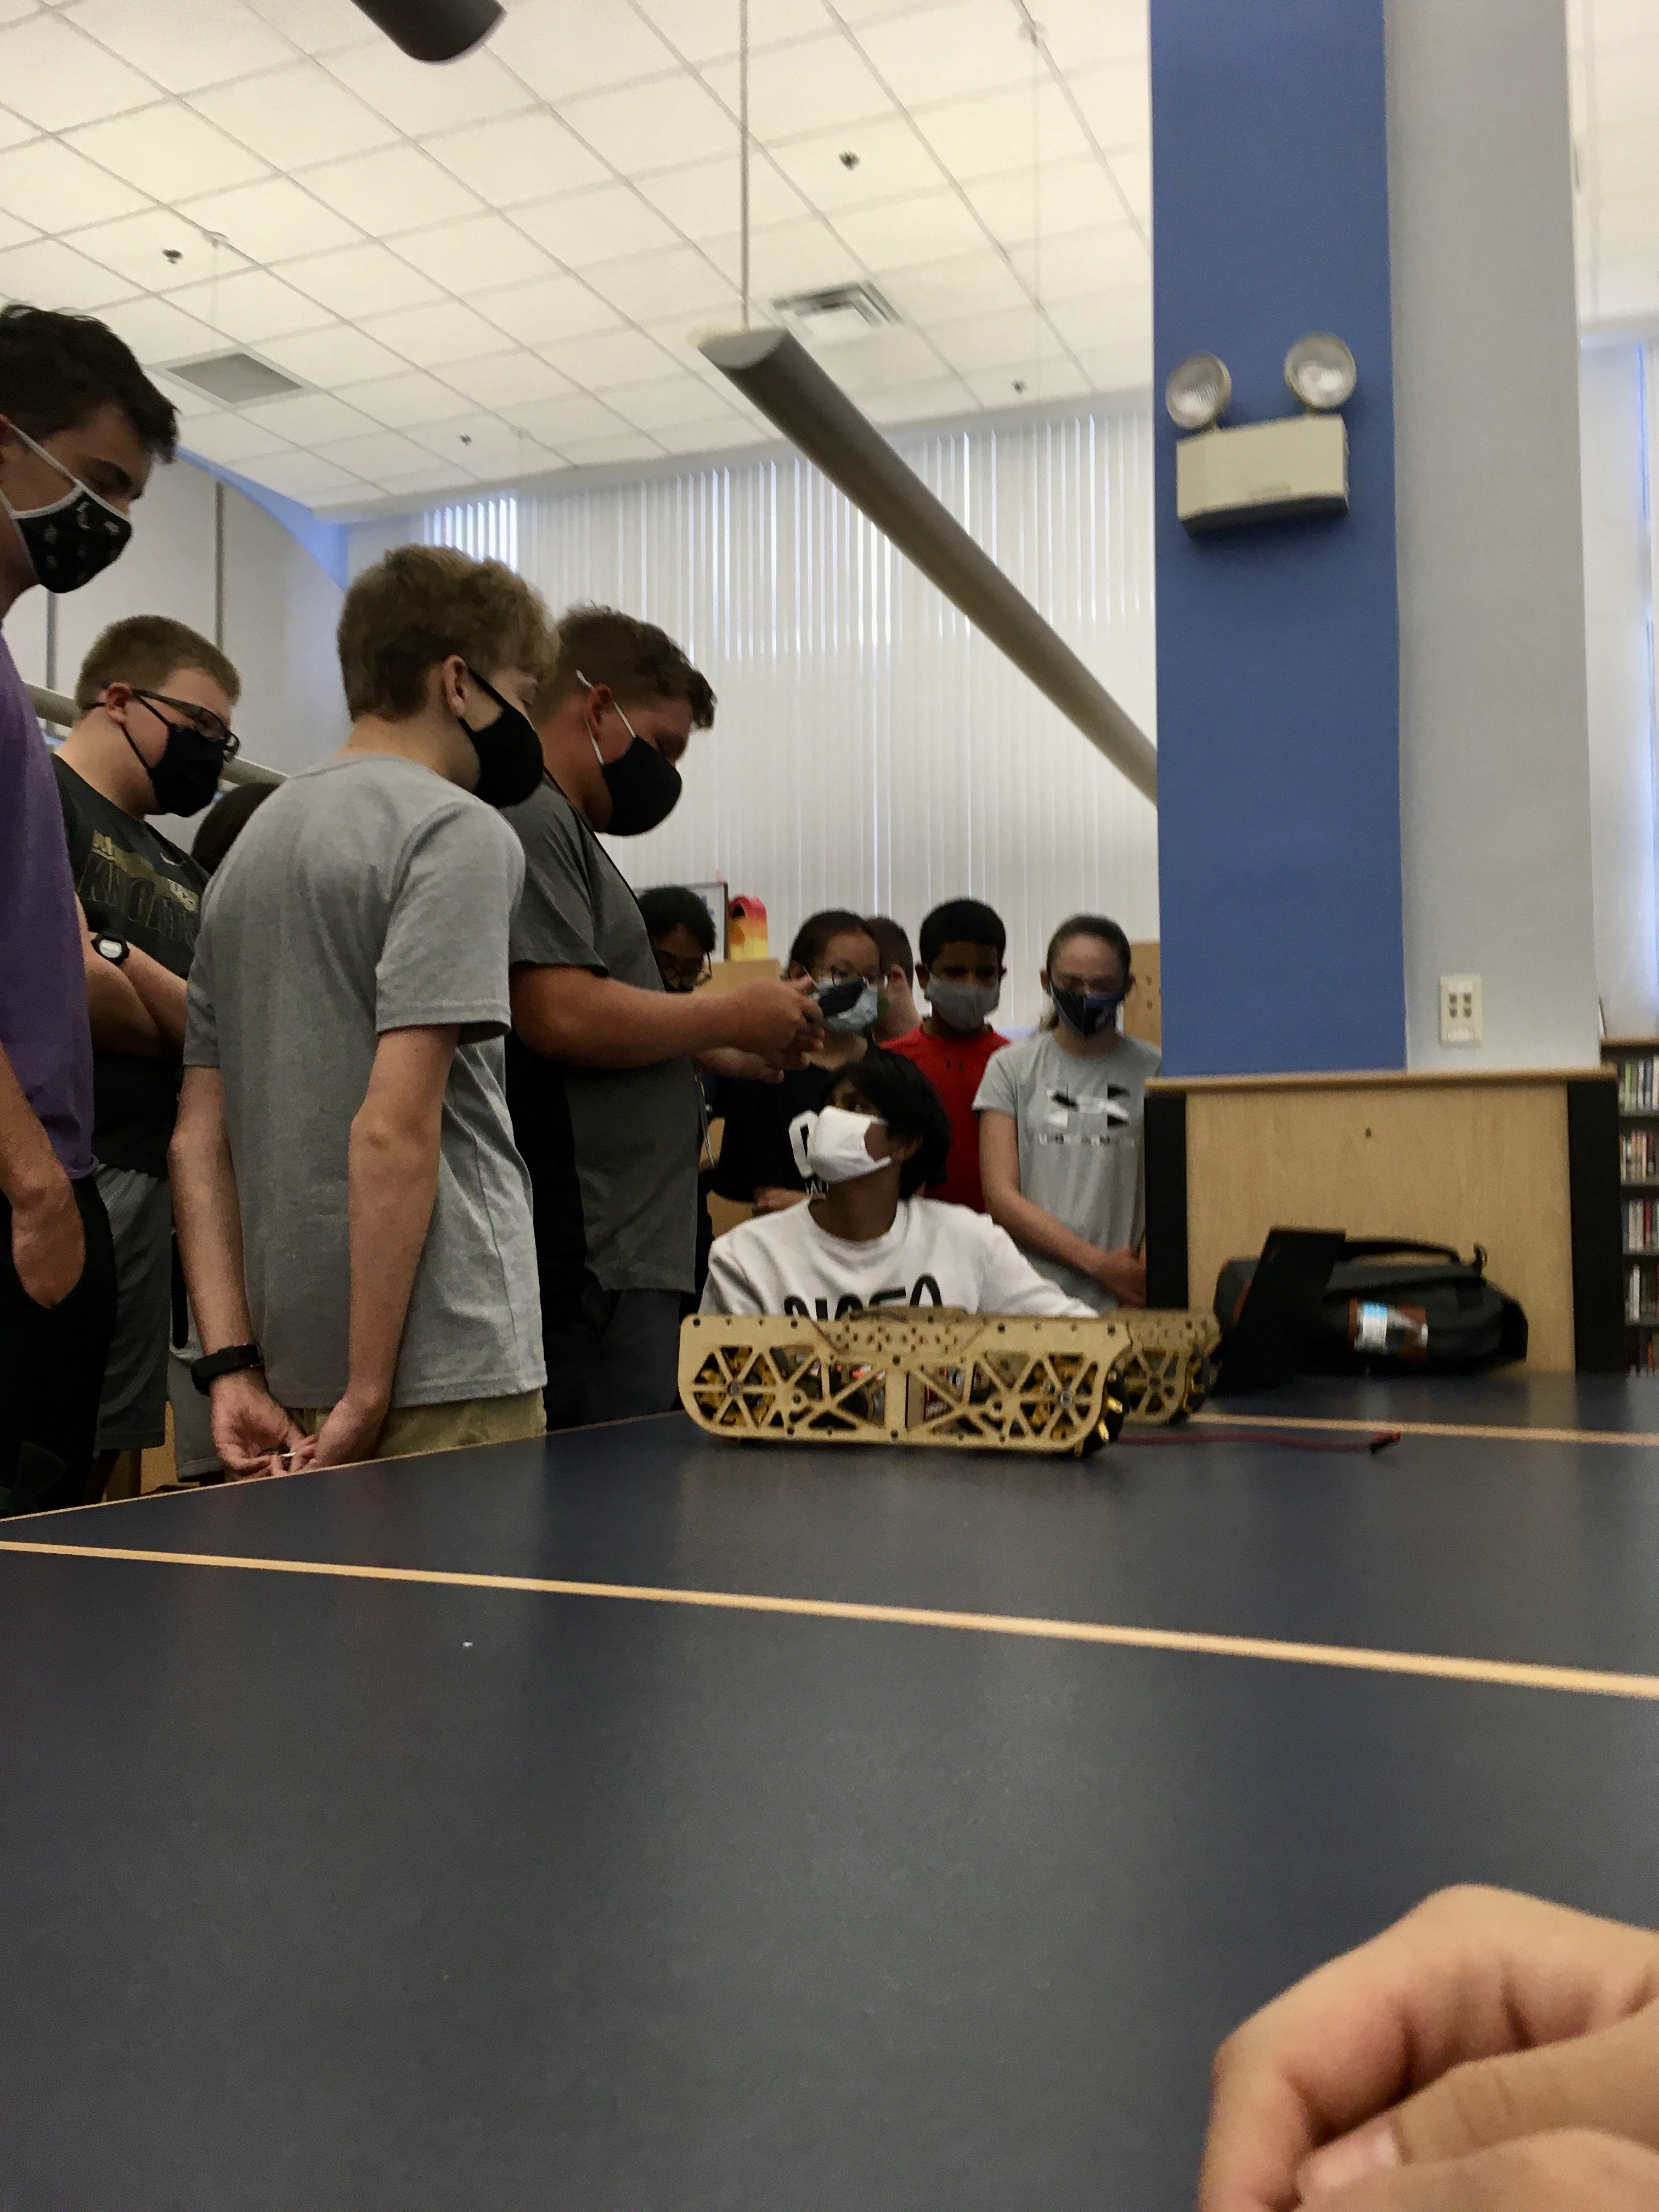
\includegraphics[width=0.9\textwidth, angle=0]{Meetings/August/08-18-21/08-18-21 1.JPG}
  \caption{Ritam helping show younger members the fundamentals of CAD.}
  \label{fig:pic1}
\end{minipage}
\begin{minipage}[b]{.50\textwidth}
  \centering
  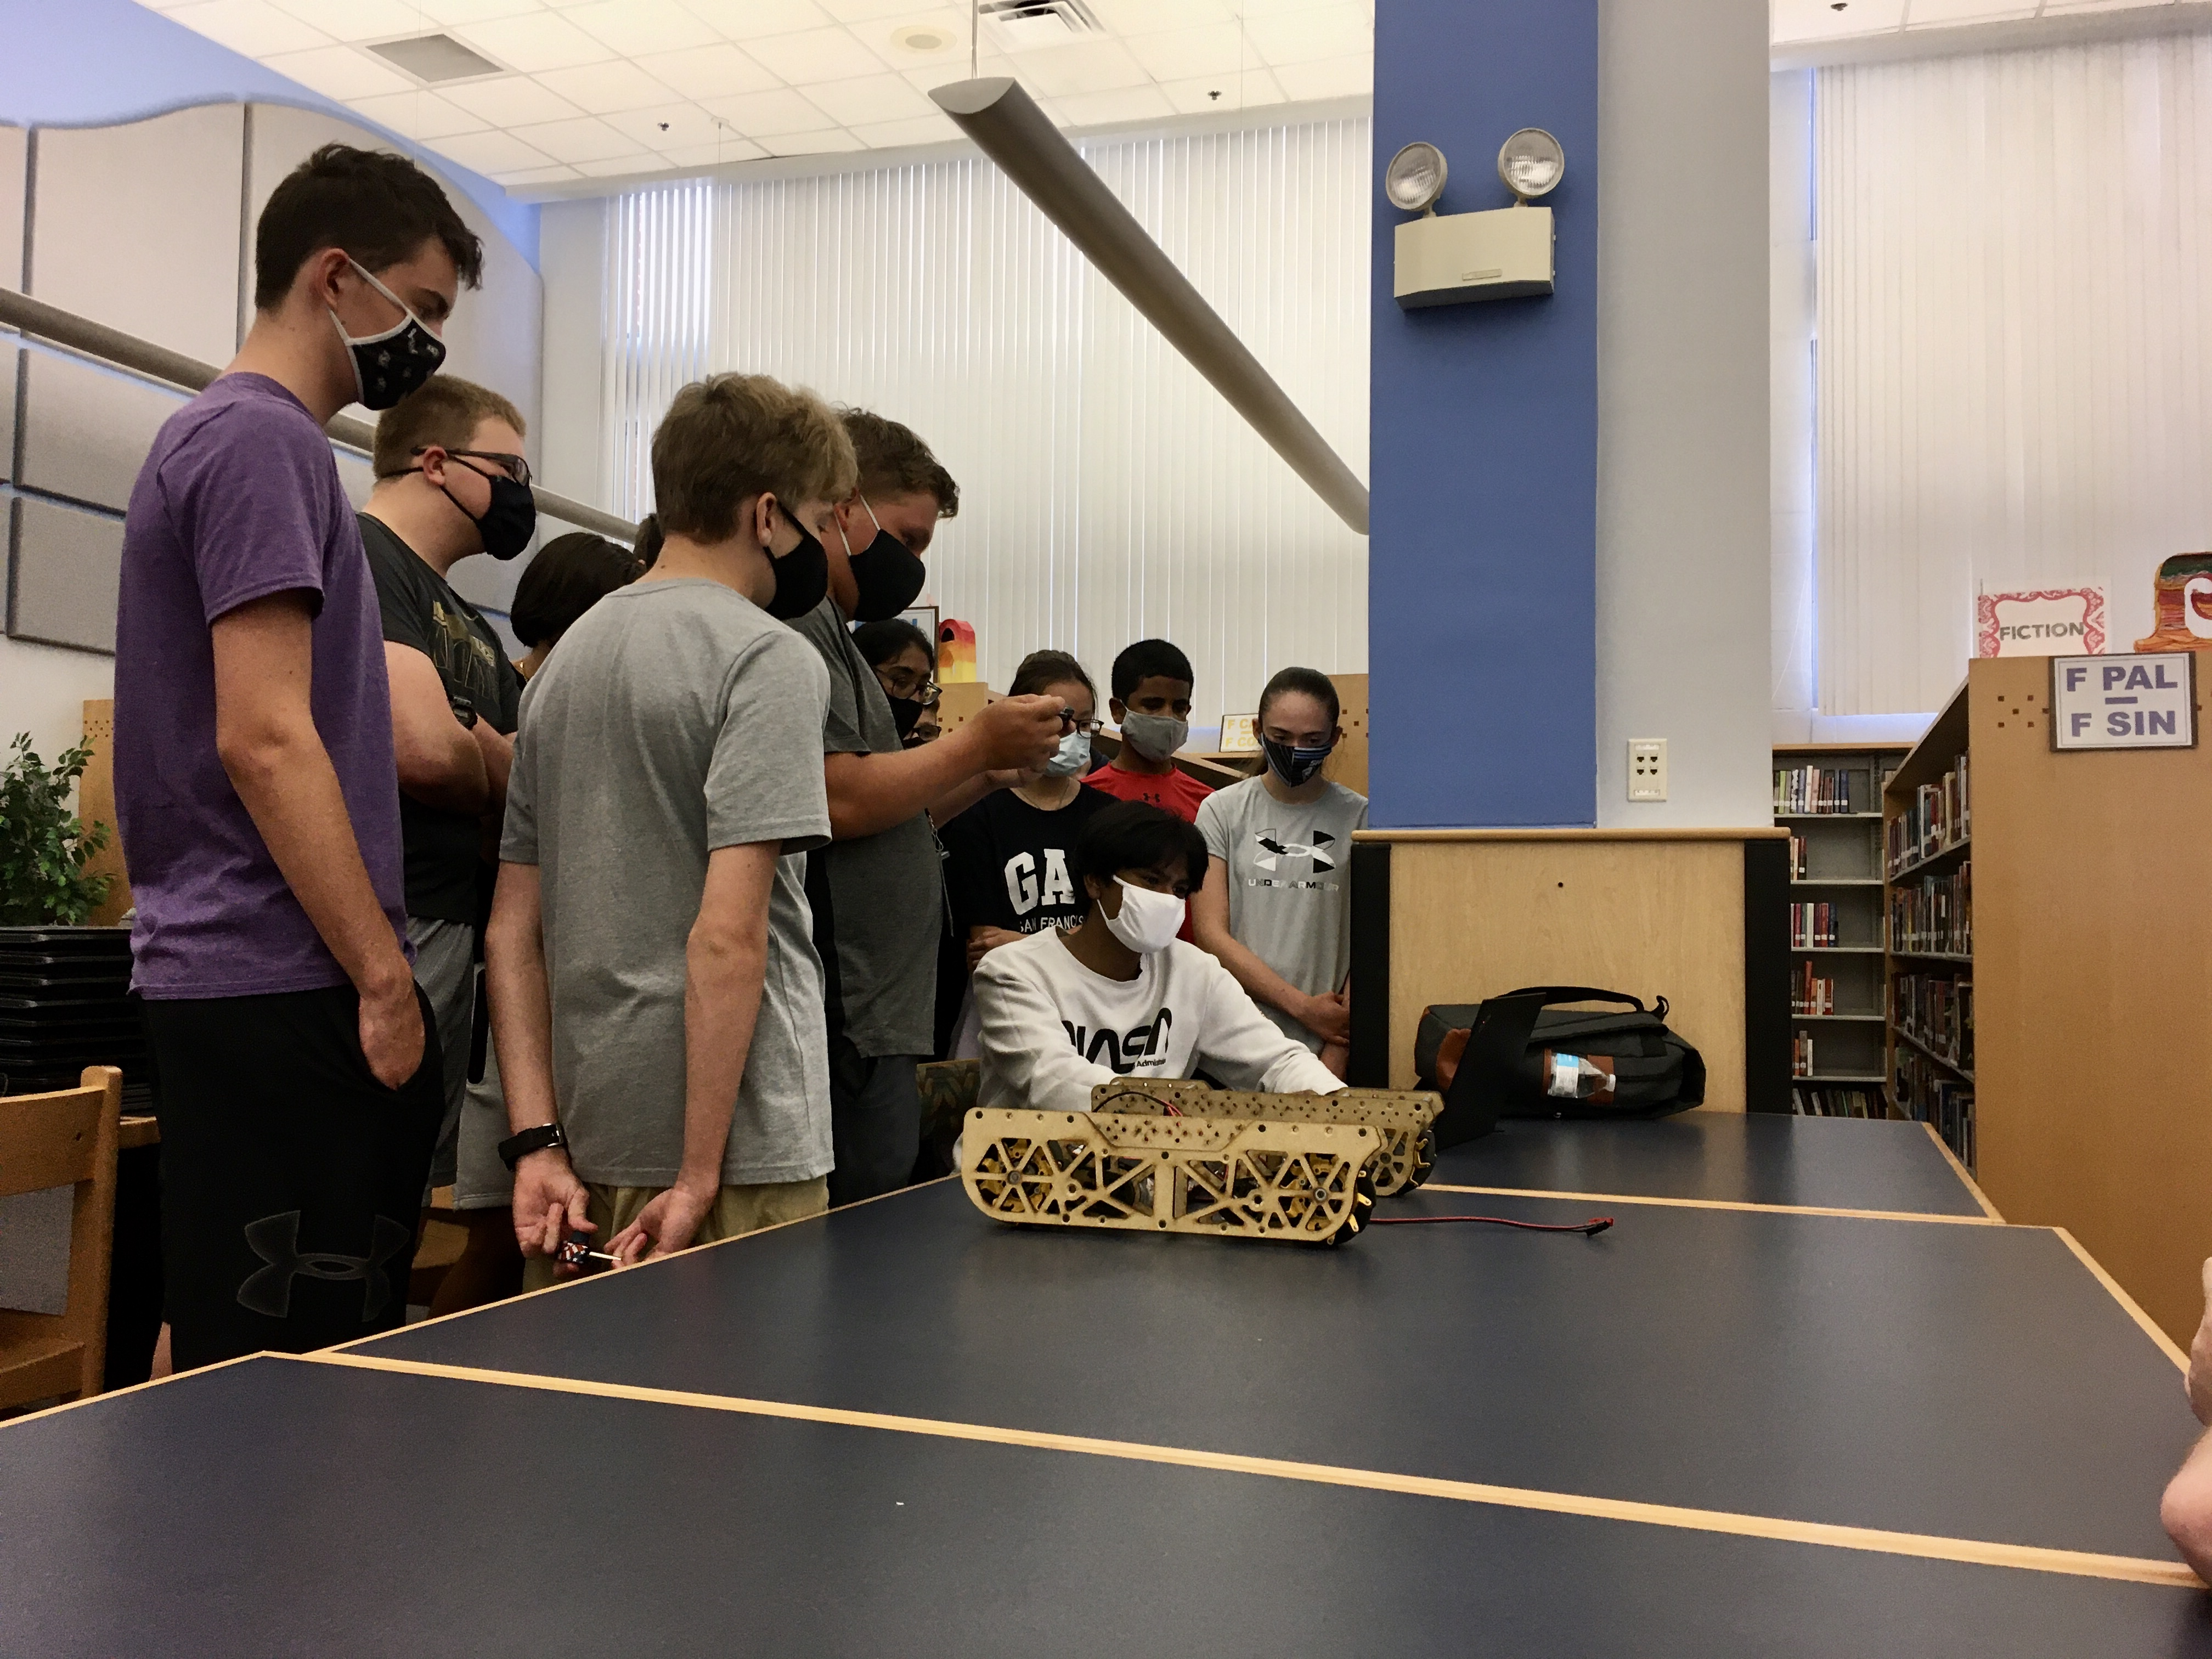
\includegraphics[width=0.9\textwidth, angle=0]{Meetings/August/08-18-21/08-18-21 2.JPG}
  \caption{More Ritam helping show younger members the fundamentals of CAD.}
  \label{fig:pic2}
\end{minipage}
\end{figure}